\documentclass[12pt]{article}
\usepackage{graphicx}
\usepackage[none]{hyphenat}
\usepackage{graphicx}
\usepackage{listings}
\usepackage[english]{babel}
\usepackage{graphicx}
\usepackage{caption} 
\usepackage{booktabs}
\usepackage{array}
\usepackage{amssymb} % for \because
\usepackage{amsmath}   % for having text in math mode
\usepackage{extarrows} % for Row operations arrows
\usepackage{listings}
\lstset{
  frame=single,
  breaklines=true
}
\usepackage{hyperref}
  
%Following 2 lines were added to remove the blank page at the beginning
\usepackage{atbegshi}% http://ctan.org/pkg/atbegshi
\AtBeginDocument{\AtBeginShipoutNext{\AtBeginShipoutDiscard}}


%New macro definitions
\newcommand{\mydet}[1]{\ensuremath{\begin{vmatrix}#1\end{vmatrix}}}
\providecommand{\brak}[1]{\ensuremath{\left(#1\right)}}
\providecommand{\norm}[1]{\left\lVert#1\right\rVert}
\providecommand{\abs}[1]{\left\vert#1\right\vert}
\newcommand{\solution}{\noindent \textbf{Solution: }}
\newcommand{\myvec}[1]{\ensuremath{\begin{pmatrix}#1\end{pmatrix}}}
\let\vec\mathbf


\begin{document}

\begin{center}
\title{\textbf{Conic Sections - Ellipse}}
\date{\vspace{-5ex}} %Not to print date automatically
\maketitle
\end{center}
\setcounter{page}{1}

\section{11$^{th}$ Maths - Chapter 11}
This is Problem-1 from Exercise 11.3
\begin{enumerate}
	\item Find the coordinates of the focii, the vertices, the length of major and minor axes, the eccentricity and the length of the latus rectum of an ellipse whose equation is given by $\frac{x^2}{36}+\frac{y^2}{16} = 1$. \\ 
\solution 
The given equation of the ellipse can be rearranged as
\begin{align}
    \label{eq:ellipseEq1}
    4x^2 + 9y^2-144 = 0
\end{align}
The above equation can be equated to the generic equation of conic sections
\begin{align}
	\label{eq:ellipseEq2}
	g\brak{\vec{x}} = \vec{x}^T\vec{V}\vec{x} + 2\vec{u}^T\vec{x} + f = 0 
\end{align}
Comparing coefficients of both equations \eqref{eq:ellipseEq1} and \eqref{eq:ellipseEq2} 
\begin{align}
	\label{eq:eqV}
	\vec{V} &= \myvec{ 4 & 0 \\ 0 & 9} \\
	\label{eq:eqU}
	\vec{u} &=  0 \\
	\label{eq:eqF}
	f &= -144 
\end{align}
From equation \eqref{eq:eqV}, since $\vec{V}$ is already diagonalized, the Eigen values $\lambda_1$ and $\lambda_2$ are given as 
\begin{align}
	\label{eq:eqEigen1}
	\lambda_1 &= 4 \\
	\label{eq:eqEigen2}
	\lambda_2 &= 9 
\end{align}
Since the given matrix is diagonal, the Eigen Vector matrix will be identity. It is given as
\begin{align}
	\vec{P} &= \myvec{ \vec{p_1} & \vec{p_2}} \\
	&= \myvec{ 1 & 0 \\ 0 & 1}
\end{align}
\begin{enumerate}
\item The eccentricity of the ellipse is given as  
\begin{align}
	e &= \sqrt{1-\frac{\lambda_1}{\lambda_2}} \\
	  &= \sqrt{1-\frac{4}{9}} \\
          &= \frac{\sqrt{5}}{3}
\end{align}
\item Finding the coordinates of Focii: 
\begin{align}
	\vec{n} &= \sqrt{\lambda_2}\vec{p_1} \\
	&= \sqrt(9)\myvec{1 \\ 0} \\
	\label{eq:eqN}
	&= \myvec{3 \\ 0} 
\end{align}
\begin{align}
	\label{eq:eqC}
	c  &=    \frac{e\vec{u}^{\top}\vec{n} \pm \sqrt{e^2\brak{\vec{u}^{\top}\vec{n}}^2-\lambda_2\brak{e^2-1}\brak{\norm{\vec{u}}^2 - \lambda_2 f}}}{\lambda_2e\brak{e^2-1}} 
\end{align}
Substituting values of $e, \vec{u}, \vec{n}, \lambda_2 \text{ and } f$ in \eqref{eq:eqC}
\begin{align}
	&=    \frac{0 \pm \sqrt{0-9\brak{\frac{5}{9}-1}\brak{{0 + 9\brak{144}}}}}{9\frac{\sqrt{5}}{3}\brak{\frac{5}{9}-1}} \\ 
	&=    \frac{ \pm 72}{-4\frac{\sqrt{5}}{3}}  \\ 
	&=    \frac{ \pm 54}{\sqrt{5}} 
\end{align}
The focus $\vec{F}$ of ellipse is expressed as
\begin{align}
	\vec{F} &= \frac{ce^2\vec{n}-\vec{u}}{\lambda_2} \\
	&= \frac{\frac{ \pm 54}{\sqrt{5}} \brak{\frac{5}{9}}\myvec{3 \\0}}{9} \\
	&= \pm \myvec{2\sqrt{5} \\ 0}
\end{align}
\item  The length of the major axis $2a$ is given by
\begin{align}
	\label{eq:majorLength}
	& 2\sqrt{\abs{\frac{f_0}{\lambda_1}}}
\end{align}
where
\begin{align}
	 f_0 &= \vec{u}^\top\vec{V}^{-1}\vec{u}-f \\
	 f_0 &= 144 \because \vec{u} = 0 \\
	\eqref{eq:majorLength} \implies  & 2\sqrt{\abs{\frac{144}{4}}}\\
	&= 12
\end{align}

\item  The length of the minor axis is given by
\begin{align}
	\label{eq:minorLength}
	& 2\sqrt{\abs{\frac{f_0}{\lambda_2}}}\\
	&= 2\sqrt{\abs{\frac{144}{9}}}\\
	&= 8
\end{align}
\item The vertices of the ellipse are given by 
\begin{align}
	& \pm\myvec{\frac{\text{2a}}{2} \\ 0} \\
	&= \pm\myvec{6 \\ 0}
\end{align}
\item The length of the latus rectum is given as 
\begin{align}
	\label{eq:eqLatRectLen}
	& 2\frac{\sqrt{\abs{f_0\lambda_1}}}{\lambda_2} \\
	&= 2\frac{\sqrt{\abs{144\brak{4}}}}{9} \\
	&= \frac{16}{3}
\end{align}
The relevant diagram is shown in Figure \ref{fig:Fig1}
\begin{figure}[!h]
	\begin{center}
		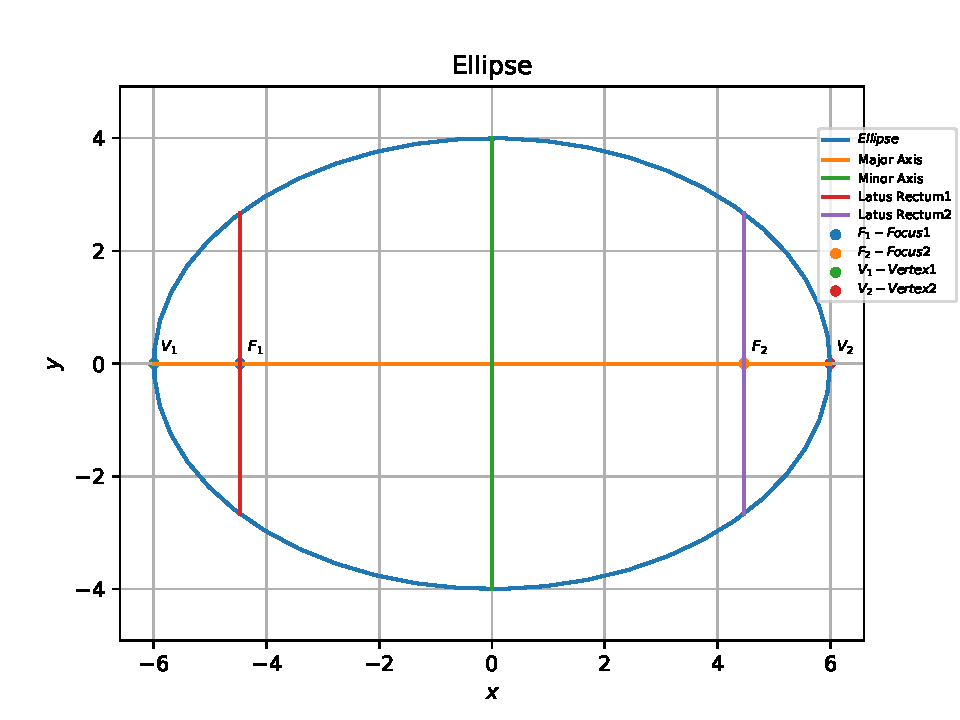
\includegraphics[width=\columnwidth]{./figs/problem1.pdf}
	\end{center}
\caption{}
\label{fig:Fig1}
\end{figure}
\end{enumerate}
\end{enumerate}
\end{document}
